% SC1005 --- Chapter 8: Memory and Programmable Logic (0->100)
\chapter{Memory and Programmable Logic}
\label{ch:memory}

\begin{quote}
\emph{``Logic computes; memory remembers across power cycles and clock cycles.''}
From one-bit cells to RAM, ROM, and the programmable fabrics that let you
\emph{draw} a circuit into existence---the storage side of digital design.
\end{quote}

\noindent\fbox{\parbox{\dimexpr\linewidth-2\fboxsep-2\fboxrule}{%
\textbf{From zero: memory from latches.} We build up from latch/register (Ch.~\ref{ch:registers})
to arrays, then show how any truth table becomes a memory lookup, and how FPGAs generalise this.}}
\vspace{0.4em}

\section*{Learning Outcomes}
After this chapter you will be able to:
\begin{enumerate}[label=(L\arabic*)]
    \item explain SRAM and DRAM cells and their tradeoffs;
    \item describe address decoding, read/write timing, and memory expansion;
    \item distinguish ROM, PROM, EPROM, EEPROM, and Flash;
    \item use PLA, PAL, and ROM as two-level logic implementations;
    \item describe FPGA organization (LUTs, interconnect, configuration).
\end{enumerate}

% ============================================================
\section{Memory Organization}
\label{sec:memory-org}
A $2^n\times m$ memory holds $2^n$ words of $m$ bits. Inputs: $n$ address lines select one word,
$m$ data lines carry the word, plus $\overline{CS}$ (chip select), $R/\bar W$ (read vs.\ write),
and $\overline{OE}$ (output enable). Internally: a matrix of cells, row/column decoders, and sense amplifiers.

Capacity examples: $1\text{K}\times8 = 8192$ bits $=1$\,KB. Address space grows exponentially with $n$;
widening $m$ replicates arrays in parallel.

\begin{figure}[h]
\centering
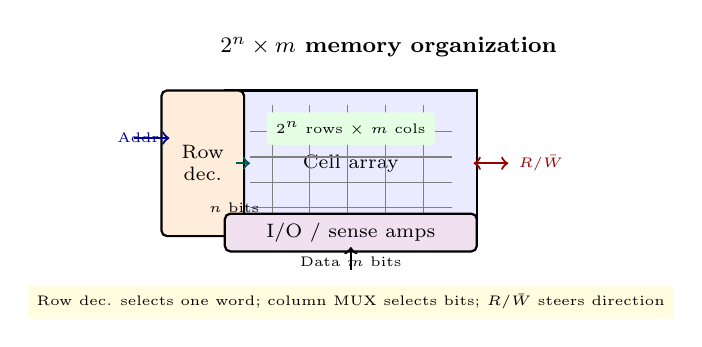
\begin{tikzpicture}[scale=0.80,every node/.style={font=\scriptsize}]
\node[font=\footnotesize\bfseries] at (3.0,3.0) {$2^n\times m$ memory organization};
% Memory array
\node[draw,thick,fill=blue!8,minimum width=3.2cm,minimum height=1.85cm] (array) at (2.4,1.15) {Cell array};
\foreach \y in {0.45,0.85,1.25,1.65} \draw[thin,gray] (0.8,\y)--(4.0,\y);
\foreach \x in {1.15,1.75,2.35,2.95,3.55} \draw[thin,gray] (\x,0.22)--(\x,2.08);
\node[font=\tiny,fill=green!10,rounded corners=1pt] at (2.4,1.70) {$2^n$ rows $\times$ $m$ cols};
% Row decoder
\node[draw,thick,fill=orange!14,minimum width=1.05cm,minimum height=1.85cm,rounded corners=2pt,align=center] (rdec) at (0.05,1.15) {Row\\dec.};
\draw[->,thick,blue!60!black] (-1.05,1.55)--(-0.48,1.55) node[left,font=\tiny] {Addr};
\draw[->,thick,teal!70!black] (0.57,1.15)--(0.80,1.15);
\node[font=\tiny] at (0.55,0.45) {$n$ bits};
% Data I/O
\node[draw,thick,fill=violet!12,minimum width=3.2cm,minimum height=0.45cm,rounded corners=2pt] (io) at (2.4,0.05) {I/O / sense amps};
\draw[->,thick] (2.4,-0.55)--(2.4,-0.18) node[below,font=\tiny] {Data $m$ bits};
\draw[<->,thick,red!60!black] (4.35,1.15)--(4.90,1.15) node[right,font=\tiny] {$R/\bar W$};
% Expansion hint
\node[font=\tiny,fill=yellow!12,rounded corners=1pt] at (2.4,-1.05) {Row dec. selects one word; column MUX selects bits; $R/\bar W$ steers direction};
\end{tikzpicture}
\caption{Memory as a matrix: address decoded to one row, data flows through sense amplifiers. Controls $R/\bar W$, $\overline{CS}$, $\overline{OE}$ gate the transfer.}
\label{fig:memory-org}
\end{figure}

\section{SRAM vs.\ DRAM Cell}
\label{sec:sram-dram}
\emph{SRAM} cell: 6-transistor bistable (cross-coupled inverters + access transistors)---fast, no refresh, larger area.
\emph{DRAM} cell: 1 transistor + 1 capacitor---tiny, dense, but charge leaks and must be refreshed every few ms,
and reads are destructive (charge sharing) so a write-back is required. SRAM for caches, DRAM for main memory.

ROM variants: mask ROM (factory), PROM (one-time fuse), EPROM (UV-erase), EEPROM/Flash (electrically erase in blocks)---non-volatile.

\section{Programmable Logic: PLA, PAL, ROM}
Any $n$-input, $m$-output combinational function is a $2^n\times m$ lookup table: address = input code,
data = output values. Using a ROM this way trades silicon for universality but wastes capacity when don't-cares abound.

\emph{PLA} (Programmable Logic Array): programmable AND plane (product terms) followed by programmable OR plane---
minimal two-level realization. \emph{PAL} (Programmable Array Logic): programmable AND, fixed OR---cheaper,
faster, slightly less flexible. Both are field-programmable (fuses/antifuses/Flash).

\begin{figure}[h]
\centering
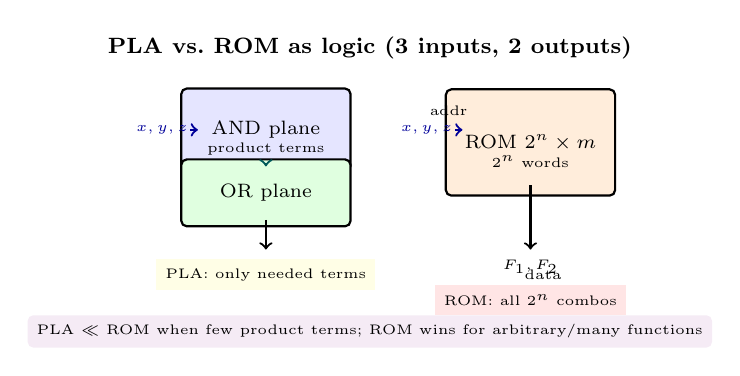
\begin{tikzpicture}[scale=0.80,every node/.style={font=\scriptsize}]
\node[font=\footnotesize\bfseries] at (3.0,2.85) {PLA vs.\ ROM as logic (3 inputs, 2 outputs)};
% PLA
\begin{scope}
\node[draw,thick,fill=blue!10,minimum width=2.15cm,minimum height=1.05cm,rounded corners=2pt] (and) at (1.35,1.55) {AND plane};
\node[font=\tiny] at (1.35,1.25) {product terms};
\node[draw,thick,fill=green!12,minimum width=2.15cm,minimum height=0.85cm,rounded corners=2pt] (or) at (1.35,0.55) {OR plane};
\draw[->,thick,blue!60!black] (0.15,1.55)--(0.27,1.55) node[left,font=\tiny] {$x,y,z$};
\draw[->,thick,teal!70!black] (1.35,1.02)--(1.35,0.97);
\draw[->,thick] (1.35,0.12)--(1.35,-0.35) node[below,font=\tiny] {$F_1,F_2$};
\node[font=\tiny,fill=yellow!10] at (1.35,-0.75) {PLA: only needed terms};
\end{scope}
% ROM
\begin{scope}[xshift=4.2cm]
\node[draw,thick,fill=orange!14,minimum width=2.15cm,minimum height=1.35cm,rounded corners=2pt] (rom) at (1.35,1.35) {ROM $2^n\times m$};
\node[font=\tiny] at (1.35,1.05) {$2^n$ words};
\draw[->,thick,blue!60!black] (0.15,1.55)--(0.27,1.55) node[left,font=\tiny] {$x,y,z$};
\node[font=\tiny] at (0.05,1.85) {addr};
\draw[->,thick] (1.35,0.67)--(1.35,-0.35) node[below,font=\tiny] {$F_1,F_2$};
\node[font=\tiny] at (1.55,-0.75) {data};
\node[font=\tiny,fill=red!10] at (1.35,-1.15) {ROM: all $2^n$ combos};
\end{scope}
% Efficiency note
\node[font=\tiny,align=center,fill=violet!8,rounded corners=2pt] at (3.0,-1.65) {PLA $\ll$ ROM when few product terms; ROM wins for arbitrary/many functions};
\end{tikzpicture}
\caption{Two ways to make any combinational function: PLA creates only the product terms you need; ROM stores the full truth table.}
\label{fig:pla-rom}
\end{figure}

\section{FPGAs: Logic You Configure}
\label{sec:fpga}
A Field-Programmable Gate Array tiles \emph{Configurable Logic Blocks} (CLBs) containing
Look-Up Tables (LUTs, typically 4--6 input SRAM memories that \emph{are} tiny ROMs), flip-flops,
and MUXes, stitched by a programmable interconnect fabric. Configuration is a bitstream loaded
from Flash/SRAM that sets every LUT truth table and every routing switch.

Design flow: HDL $\to$ synthesis $\to$ mapping to LUTs $\to$ place \& route $\to$ bitstream.
Reprogrammable in milliseconds---prototyping, acceleration, and low-volume production.

\begin{figure}[h]
\centering
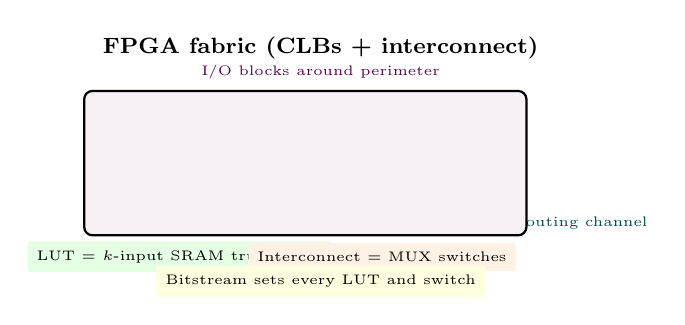
\begin{tikzpicture}[scale=0.78,every node/.style={font=\scriptsize}]
\node[font=\footnotesize\bfseries] at (3.5,2.85) {FPGA fabric (CLBs + interconnect)};
\foreach \x in {0,1,2,3} {
  \foreach \y in {0,1,2} {
    \pgfmathsetmacro{\px}{\x*1.55}
    \pgfmathsetmacro{\py}{\y*0.62+0.15}
    \node[draw,thick,fill=blue!\the\numexpr 10+\y*5\relax,minimum width=1.15cm,minimum height=0.48cm,rounded corners=1pt] at (\px+0.68,\py) {CLB};
    \node[font=\tiny] at (\px+0.68,\py) {LUT+FF};
  }
}
% Interconnect channels
\draw[thick,teal!60!black,dashed] (-0.15,0.0)--(6.55,0.0) node[right,font=\tiny] {routing channel};
\draw[thick,teal!60!black,dashed] (-0.15,0.62)--(6.55,0.62);
\draw[thick,teal!60!black,dashed] (-0.15,1.24)--(6.55,1.24);
% Labels
\node[font=\tiny,fill=green!10,rounded corners=1pt] at (1.2,-0.55) {LUT = $k$-input SRAM truth table};
\node[font=\tiny,fill=orange!10,rounded corners=1pt] at (4.5,-0.55) {Interconnect = MUX switches};
\node[font=\tiny,fill=yellow!12] at (3.5,-0.95) {Bitstream sets every LUT and switch};
% I/O ring
\draw[thick,rounded corners=3pt,fill=violet!6] (-0.35,-0.20) rectangle (6.85,2.15);
\node[font=\tiny,violet!70!black] at (3.5,2.45) {I/O blocks around perimeter};
\end{tikzpicture}
\caption{FPGA: array of CLBs (each a LUT plus optional flip-flop) connected by a programmable routing fabric. The bitstream configures LUT contents and interconnect.}
\label{fig:fpga}
\end{figure}

Memory hierarchy note: registers (fastest, fewest), SRAM caches, DRAM main memory, Flash/SSD storage---each level trades speed for capacity and cost. Temporal and spatial locality make the hierarchy effective.


\section{Read/Write Timing and Memory Expansion}
Read cycle: place address, assert $\overline{CS}$ and $\overline{OE}$, wait $t_{AA}$ (address access time), sample data.
Write cycle: place address and data, pulse $\overline{WE}$ or $R/\bar W$, meet setup/hold $t_{AS},t_{DS},t_{DH}$. SRAM is asynchronous
or synchronous (clocked, pipelined for cache). DRAM needs $\overline{RAS}/\overline{CAS}$ multiplexing and periodic refresh
(burst or distributed, $\sim64$\,ms retention).

Expansion: widening ($m$) parallels chips sharing address; deepening ($2^n$) decodes upper address bits to chip-selects.
Example: $4\text{K}\times8$ from $1\text{K}\times8$ needs $4$ chips, $2$ address bits into a 2-to-4 decoder whose outputs are $\overline{CS}_i$,
data buses tied together (tri-state or wired-OR with $\overline{OE}$ gating).
\begin{example}[ROM as lookup]
A $32\times8$ ROM stores ASCII codes: address $=5$-bit input code, data $=8$-bit ASCII. Changing the function is a ROM reprogram,
not a rewiring---the original ``firmware'' idea before Flash and FPGAs made reconfiguration routine.
\end{example}

% ============================================================

% ============================================================
\section{Chapter Notes}
Wilkes (EDSAC, 1949) introduced stored-program memory; Dennard's 1T DRAM (1968) enabled cheap main memory.
PLAs/PALs dominated glue logic in the 1980s; Xilinx XC2064 (1985) launched the FPGA era (now AMD/Xilinx and Intel/Altera).

% ============================================================
\section{Memory Hierarchy and Locality}
Registers ($t\sim0.3$\,ns) $\to$ SRAM cache ($1$--$3$\,ns) $\to$ DRAM ($50$--$100$\,ns) $\to$ Flash/SSD ($50\,\mu$s--$1$\,ms) $\to$ disk.
Each level is larger, cheaper per bit, and slower. \emph{Temporal locality} (reuse) and \emph{spatial locality} (nearby addresses)
make caches effective: a small fast cache captures most accesses. Write policies (write-through vs.\ write-back) and replacement
(LRU) manage coherence between levels---full treatment in computer architecture (SC1007/SC2002).

% ============================================================

\paragraph{Error detection.} Memories add parity or ECC: single-bit parity detects one error; Hamming $(72,64)$
corrects one bit and detects two (SECDED) with 8 check bits per 64-bit word---standard in servers. Flash adds wear
leveling and bad-block management since cells degrade after $\sim10^5$ program/erase cycles; the controller remaps
writes to spread wear, turning the memory into a small computer itself.

\paragraph{Non-volatile evolution.} Mask ROM gave way to PROM (fusible links), EPROM (floating-gate, UV erase), EEPROM
(byte-erase via Fowler--Nordheim tunneling), and Flash (block-erase, NOR for XIP vs.\ NAND for density). Emerging NVM---MRAM,
ReRAM, PCM---promise DRAM-like speed with non-volatility, potentially collapsing the memory hierarchy in future architectures.
Resistance and endurance remain active research frontiers.

\paragraph{Programmable logic in modern flows.} HDL synthesis maps \texttt{case} and \texttt{if}--\texttt{else} to MUXes and LUTs automatically;
the designer rarely instantiates PLA/PAL explicitly. Yet understanding them explains why a 4-LUT FPGA needs $\lceil n/4\rceil$ LUTs
per $n$-input function and why wide AND-OR structures benefit from dedicated carry/AND chains in modern FPGAs (e.g.\ Xilinx CARRY4).

\section{Exercises}
\label{sec:ch08-exercises}
\begin{enumerate}[label=E8.\arabic*, leftmargin=*, itemsep=0.8em]
    \item \textbf{SRAM vs.\ DRAM.} Compare 6T SRAM and 1T1C DRAM on transistor count, speed, refresh, and use case. Why is DRAM destructive on read?
    \item \textbf{Expansion.} Build $2\text{K}\times8$ from $1\text{K}\times8$ chips. How many chips? Draw address and data wiring, including $\overline{CS}$ decoding.
    \item \textbf{ROM logic.} Implement $F=\sum m(1,2,5,6)$ and $G=\sum m(0,3,7)$ (3 inputs) using an $8\times2$ ROM. List ROM contents. Repeat with a PLA using minimal product terms.
    \item \textbf{LUT mapping.} A 4-LUT can realise any 4-input function. How many 4-LUTs are needed for a 6-input AND? For a 4-bit adder's sum bits? Sketch the mapping.
    \item \textbf{Flash vs.\ EEPROM.} Distinguish NOR and NAND Flash on erase granularity, random access, and typical application (code storage vs.\ data storage).
\end{enumerate}
% End of Chapter 8
